\chapter{Software Development Life Cycle \& Process Models}
\label{ch:sdlc}

Software engineering exists because building software at scale is not just coding. A single developer can hack together a hundred-line script in an afternoon. A team of fifty building a banking system for millions of users needs discipline, predictability, and quality assurance. The \emph{Software Development Life Cycle} (SDLC) provides that structure, and the choice of process model determines how risk, cost, and time are managed.

\section{What Is Software Engineering?}

\begin{definition}[Software Engineering]
The systematic application of engineering principles to the design, development, maintenance, testing, and evaluation of software and systems.
\end{definition}

The term was coined at NATO's 1968 conference during the so-called \emph{software crisis}: projects were late, over budget, and unreliable. The crisis has not disappeared---it has scaled. Modern systems are distributed, concurrent, security-critical, and continuously evolving. Engineering discipline is what separates a prototype from a product that can be operated safely for a decade.

Key characteristics of engineered software include:
\begin{itemize}
    \item \textbf{Maintainability} --- can be understood and modified by people other than the original authors.
    \item \textbf{Reliability and availability} --- fails rarely, degrades gracefully, and recovers without data loss.
    \item \textbf{Efficiency} --- uses time, memory, and energy within acceptable bounds.
    \item \textbf{Usability and security} --- meets user needs while protecting assets and privacy.
    \item \textbf{Traceability} --- every artefact can be traced from requirement to code to test.
\end{itemize}

Software engineering is not just process; it is economics. Boehm's classic data shows that fixing a requirements defect during maintenance costs $100\times$ more than fixing it during requirements. Process exists to catch defects early.

\section{Phases of the SDLC}

Every SDLC model organises the same fundamental phases, differing only in sequencing, iteration, and feedback:

\begin{enumerate}
    \item \textbf{Requirement analysis} --- what must the system do and how well?
    \item \textbf{System and software design} --- architecture, components, interfaces, data models.
    \item \textbf{Implementation (coding)} --- translating design into executable code.
    \item \textbf{Testing and verification} --- does the system meet its specification?
    \item \textbf{Deployment and release} --- delivering the system to its operational environment.
    \item \textbf{Maintenance and evolution} --- correcting faults, adapting to new needs, improving qualities.
\end{enumerate}

Although listed linearly, real projects revisit earlier phases constantly. A test failure sends you back to design; a deployment constraint forces a requirement renegotiation. The diagram below captures this iterative reality.

\begin{figure}[h]
\centering
\begin{tikzpicture}[scale=0.78, every node/.style={font=\small}]
  \def\r{2.25}
  \foreach \i/\col/\txt in {0/blue!20/Requirements,60/green!20/Design,120/orange!20/Implementation,180/violet!20/Testing,240/red!15/Deployment,300/teal!20/Maintenance} {
    \node[draw,circle,fill=\col,minimum size=2.05cm,align=center,thick] at (\i:\r) {\txt};
  }
  \foreach \a in {0,60,120,180,240,300} {
    \draw[-{Stealth[length=3mm]},thick,blue!55!black] (\a:\r) -- (\a+60:\r);
  }
  \node[align=center,font=\footnotesize\itshape,fill=yellow!10,draw,rounded corners,inner sep=3pt] at (0,0) {Iterate\\\& Feedback};
  \draw[dashed,gray,->] (0,0) -- (0.9,0.9);
\end{tikzpicture}
\caption{SDLC as an iterative cycle -- every phase feeds back to predecessors; the centre reminds us that iteration is the norm, not the exception.}
\end{figure}

\section{Classical Process Models}

\subsection{Waterfall Model}

The waterfall flows strictly top-down: each phase must complete and be signed off before the next begins. It is document-driven and easy to manage---ideal when requirements are stable and well understood, such as safety-critical embedded systems or regulatory reporting platforms.

Strengths: simple to understand, clear milestones, thorough documentation supports audits. Weaknesses: working software appears only at the end; late discovery of requirement errors is enormously expensive; customer feedback is delayed.

\begin{figure}[h]
\centering
\begin{tikzpicture}[scale=0.72, every node/.style={font=\footnotesize}]
  \tikzstyle{phase}=[draw,rounded corners,fill=blue!12,minimum width=3.4cm,minimum height=0.85cm,align=center,thick]
  \node[phase,fill=blue!15] (r) at (0,4.2) {Requirements};
  \node[phase,fill=green!15] (d) at (0,3.0) {Design};
  \node[phase,fill=orange!15] (i) at (0,1.8) {Implementation};
  \node[phase,fill=violet!15] (t) at (0,0.6) {Testing};
  \node[phase,fill=red!12] (m) at (0,-0.6) {Deployment \& Maintenance};
  \draw[-{Stealth},thick] (r) -- (d);
  \draw[-{Stealth},thick] (d) -- (i);
  \draw[-{Stealth},thick] (i) -- (t);
  \draw[-{Stealth},thick] (t) -- (m);
  \draw[{Stealth}-{Stealth},dashed,thick,gray] (t.east) -- ++(1.4,0) |- (r.east) node[midway,right,font=\tiny,align=left] {costly\\rework};
  \node[draw,fill=yellow!15,rounded corners,font=\tiny,align=center,inner sep=4pt] at (5.2,1.6) {V-Model\\extension:\\each dev phase\\has matching\\test phase};
  \draw[dashed,->,gray] (5.2,2.2) -- (0.4,3.0);
  \draw[dashed,->,gray] (5.2,1.0) -- (0.4,0.6);
\end{tikzpicture}
\caption{Waterfall flow with the costly feedback arc; the V-model mirrors each development phase (requirements, design) with a corresponding test level (acceptance, integration, unit).}
\end{figure}

The \textbf{V-model} is waterfall's disciplined sibling: it pairs each development phase with a test phase (requirements $\leftrightarrow$ acceptance test, high-level design $\leftrightarrow$ system test, detailed design $\leftrightarrow$ integration test, coding $\leftrightarrow$ unit test). This encourages early test planning and traceability.

\subsection{Incremental and Iterative Models}

Instead of one big delivery, \emph{incremental} development ships the system in slices: increment~1 delivers core features (e.g., login + catalogue), increment~2 adds checkout, increment~3 adds recommendations. Each increment is a complete, usable subset. \emph{Iterative} development refines the whole system through repeated cycles; the first iteration may be a rough prototype that is progressively hardened. In practice most projects combine both: incrementally add scope while iteratively refining quality.

Benefits include early value delivery, early feedback, and reduced risk. The cost is more complex integration and the need for a stable architecture that can accommodate future increments.

\subsection{Spiral Model}

Boehm's spiral (1988) is explicitly \emph{risk-driven}. Each loop around the spiral has four quadrants: (1) determine objectives and constraints, (2) identify and resolve risks (often via prototypes or simulations), (3) develop and test the next increment, (4) plan the next iteration. The radius represents cumulative cost; the angular dimension represents progress.

\begin{figure}[h]
\centering
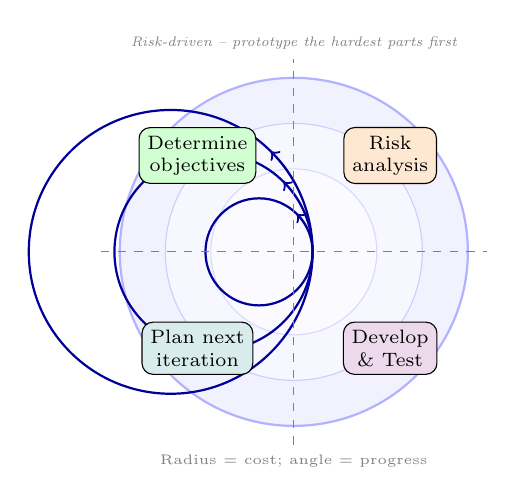
\begin{tikzpicture}[scale=0.68, every node/.style={font=\scriptsize}]
  \draw[fill=blue!5,draw=blue!30,thick] (0,0) circle (3.25cm);
  \draw[fill=blue!3,draw=blue!20] (0,0) circle (2.4cm);
  \draw[fill=blue!2,draw=blue!15] (0,0) circle (1.55cm);
  \draw[->,thick,blue!60!black] (0.35,0) arc (0:405:1.0cm);
  \draw[->,thick,blue!60!black] (0.35,0) arc (0:405:1.85cm);
  \draw[->,thick,blue!60!black] (0.35,0) arc (0:405:2.65cm);
  \draw[dashed,gray] (-3.6,0) -- (3.6,0);
  \draw[dashed,gray] (0,-3.6) -- (0,3.6);
  \node[fill=green!18,draw,rounded corners,align=center,inner sep=3pt] at (-1.8,1.8) {Determine\\objectives};
  \node[fill=orange!18,draw,rounded corners,align=center,inner sep=3pt] at (1.8,1.8) {Risk\\analysis};
  \node[fill=violet!15,draw,rounded corners,align=center,inner sep=3pt] at (1.8,-1.8) {Develop\\ \& Test};
  \node[fill=teal!15,draw,rounded corners,align=center,inner sep=3pt] at (-1.8,-1.8) {Plan next\\iteration};
  \node[font=\tiny\itshape,gray] at (0,3.9) {Risk-driven -- prototype the hardest parts first};
  \node[font=\tiny,gray] at (0,-3.9) {Radius = cost; angle = progress};
\end{tikzpicture}
\caption{Spiral model: each cycle addresses the highest remaining risk with a prototype or analysis before committing to build. Early cycles may be paper prototypes; later cycles are production increments.}
\end{figure}

Spiral suits large, high-risk, unprecedented systems (aerospace, novel platforms) where risk analysis justifies the overhead. For routine business systems it is often too heavy.

\subsection{Choosing a Model}

\begin{table}[h]
\centering\small
\begin{tabular}{@{}lcccc@{}}
\toprule
Model & Req.\ stability & Risk handling & Delivery & Overhead \\ \midrule
Waterfall & Stable/fixed & Low & Single & Low \\
V-Model & Stable + safety-critical & Medium & Single & Medium \\
Incremental & Evolving & Medium & Multiple & Medium \\
Spiral & Highly uncertain & High (explicit) & Multiple + prototypes & High \\
Agile (Ch.~8) & Volatile & Continuous & Continuous & Low--Medium \\
\bottomrule
\end{tabular}
\caption{Guidance for selecting a process model. No single model fits all projects; hybrids are common (e.g., incremental with spiral risk analysis).}
\end{table}

A useful heuristic: if you can write a complete SRS on day one, waterfall/V-model may suffice. If you expect requirements to change weekly, choose incremental/iterative or agile. If failure could cost lives or billions, add spiral-style risk analysis regardless of other choices.


\section{Unified Process and Iterative Refinement}

The Unified Process (UP) -- and its agile descendant OpenUP -- organises development into four phases (Inception, Elaboration, Construction, Transition), each containing multiple iterations that each deliver an executable increment. Unlike waterfall, UP is architecture-centric and risk-driven: the elaboration phase builds an executable architectural prototype that tackles the highest risks before full construction begins.

\begin{itemize}
    \item \textbf{Inception} --- scope the project, identify key stakeholders and risks, produce a vision and rough estimate. Go/no-go decision.
    \item \textbf{Elaboration} --- stabilise architecture, resolve top risks, produce an executable baseline. Most requirements are now understood.
    \item \textbf{Construction} --- incrementally build the remaining features, continuously integrating and testing.
    \item \textbf{Transition} --- beta testing, deployment, user training, and handover.
\end{itemize}

UP makes explicit that disciplines (requirements, design, implementation, testing, project management) run in parallel with varying intensity across phases, rather than as strict sequential gates. Early phases are requirements-heavy; later phases are implementation-heavy. This two-dimensional view (phases $\times$ disciplines) is more realistic than any one-dimensional waterfall chart.

\section{Process Tailoring and Maturity}

No process should be adopted verbatim. Teams tailor by selecting practices that fit context: a five-person startup omits formal change-control boards, while a medical-device team cannot omit traceability audits. Capability Maturity Model Integration (CMMI) provides five maturity levels -- Initial, Managed, Defined, Quantitatively Managed, Optimising -- to assess and improve process capability. Higher maturity correlates with predictable cost and schedule, but dogmatic adherence without judgement is counter-productive.

\section{Summary}

SDLC models are tools, not religions. Waterfall suits well-understood, regulated domains; spiral suits high-risk R\&D; incremental/iterative suits most commercial software. The unifying insight is that process must be chosen deliberately, tailored to context, and continuously improved via retrospectives and metrics. Chapter~8 returns to agile and DevOps as the modern synthesis.


\section{Case Study: Choosing for a University System}

Consider NTU's course-registration system (STARS). Requirements are largely stable (enrolment rules change slowly), but performance under flash-crowd load is critical and failure during add/drop is highly visible. A pure waterfall would delay load testing until the end, risking a catastrophic bottleneck. An incremental approach that delivers registration for one school first, load-tests it with synthetic traffic, and then scales to all schools de-risks the critical quality attribute early. This illustrates that process choice should be driven by the highest risk, not by habit.

\begin{remark}
There is no universally best process. The best process is the one your team understands, tailors honestly, and improves continuously. Ceremony should be proportional to risk.
\end{remark}


\section{Process Metrics and Improvement}

What gets measured gets improved. Useful process metrics include velocity (story points per iteration), lead time (idea to production), defect density (bugs per KLOC), and escaped defects (bugs found after release). Retrospectives turn metrics into action: the team inspects data, identifies one or two improvement experiments, and reviews them next cycle. Without measurement, process ``improvement'' is just opinion.


\begin{remark}
Process tailoring example: a research spike to evaluate a new ML library needs no formal SRS, just a time-boxed experiment and a decision log. Applying full waterfall there would waste weeks.
\end{remark}

\section{Exercises}

\begin{exercise}
A hospital management system has fixed regulatory requirements but the customer insists on seeing a working prototype of the patient-record module in month~2. Which SDLC model(s) would you recommend and why? Contrast waterfall and spiral for this scenario.
\end{exercise}

\begin{exercise}
Explain why the cost of fixing a requirements defect grows exponentially across SDLC phases. Sketch the cost curve (x = phase, y = relative cost) and give a concrete example of a defect caught in testing versus one caught in maintenance.
\end{exercise}

\begin{exercise}
Distinguish incremental from iterative development. Give an example where a team does one without the other, and an example where both are combined (as in the Unified Process).
\end{exercise}

\begin{exercise}
The V-model pairs each development phase with a test phase. List the four pairings and explain what each test level validates. When does V-model outperform pure waterfall, and what is its main limitation?
\end{exercise}

\begin{exercise}
A startup building a social-media app has volatile requirements and needs to ship an MVP in 8~weeks. Argue why a plan-driven model would fail here and outline an alternative process with two increments and specific deliverables per increment.
\end{exercise}
